\begin{frame}{Motivation}
  Combinatorial Optimization problems that often emerge in real-world scenarios:
  \begin{itemize}
    \item Are~\textbf{large} and~\textbf{complex}.
    \item \textbf{Cannot be solved} by~\alert{exact} methods in a~\textbf{reasonable amount of time}.
  \end{itemize}

  The~\alert{Google Hash Code} programming competition invited people
  to solve challenging problems.

  \begin{itemize}
    \item \textbf{Complex problems} inspired by engineering challenges.
    \item Inspired by~\textbf{real-world} scenarios.
    \item \textbf{Well formulated} and can be solved to some extent in a short amount of time.
  \end{itemize}
\end{frame}

\begin{frame}{Motivation}
  \alert{Meta-Heuristics} are methods that~\textquote{guide and intelligently combine subordinate
    heuristics for exploring and exploiting solutions in the search
    space}~(\cite{osman1996metaheuristics}).

  These methods have interesting properties:
  \begin{itemize}
    \item Can often~\textbf{find~\textquote{good} solutions} for hard problems~\textbf{quickly}.
    \item \textbf{General-purpose}, i.e. they can be applied to many problems.
  \end{itemize}

  There is a community interest in studying them and making them more accessible in practice.
\end{frame}

\begin{frame}{Motivation}
  \alert{Modeling} is the process of creating a simplified representation
  or approximation of a real-world system, process, or phenomenon.

  If this process is done in a principled way, it can be standardized in order to provide:
  \begin{itemize}
    \item A~\textbf{structured approach} to problem-solving.
    \item A clear~\textbf{separation} between~\textbf{problems} and~\textbf{solvers}.
  \end{itemize}

  \begin{figure}[h]
    \centering
    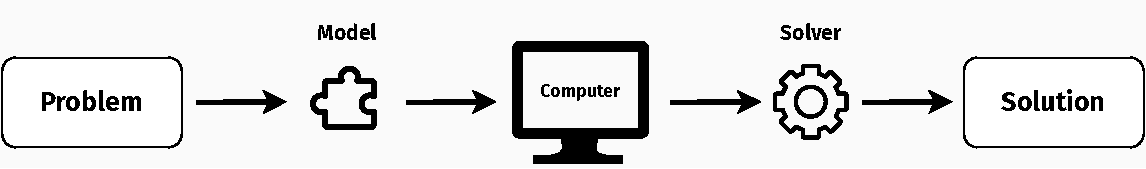
\includegraphics[width=\textwidth,keepaspectratio]{../assets/modelling/modelling-slides.pdf}
    \caption{Principled Modeling Framework}
  \end{figure}
\end{frame}

\begin{frame}{Goals \& Scope}
  The main research questions we outline for this work are:
  \begin{enumerate}
    \item Can existing ideas on modeling frameworks~(\cite{vieira2009uma,fonseca2021nasf4nio,outeiro2021application})
          be formalized into a more practical and complete implementation?

    \item Can general-purpose meta-heuristic solvers be developed
          through the principled modeling framework implementation?

    \item Can Google Hash Code problems be solved effectively using
          this modeling approach?
  \end{enumerate}
\end{frame}

\begin{frame}{Contributions}
  The main contributions of this work are related to the aforementioned research questions, as follows:
  \begin{enumerate}
    \item A practical Python implementation of the principled modeling framework was
          created.

    \item Several meta-heuristic solvers and utilities were developed on top of
          the principled modeling framework implementation.

    \item Several models were developed for two of the Google Hash Code problems.
  \end{enumerate}
\end{frame}

% TODO: Other Contributions